\documentclass[handout]{beamer}
\usepackage[utf8]{inputenc}
\usepackage[english]{babel}
\usepackage{helvet}
\usepackage[T1]{fontenc}
\usepackage{textcomp}
\usepackage[inline]{asymptote}
\usepackage{slide_helper}
\usepackage{multirow}
\usepackage{pgf-pie}
\usepackage{tikz}
\usepackage{subfigure}
\usetikzlibrary{shapes.geometric, arrows}
\usepackage{pgfplots}
\pgfplotsset{compat=1.5} 
\usepgfplotslibrary{statistics}
\usetikzlibrary{external}
\tikzexternalize%

\title[MA205 - Section 2.2]{Considering Categorical Data}

\definecolor{legend}{rgb}{0.9, 0.95, 0.9}

\begin{document}
\begin{frame}
\titlepage
\end{frame}

\begin{frame}
\begin{example}\label{contingency table}
\vspace{-2mm}%beamer bug: extra space is added when a label is used, so this is to make this slide and the next look the same
The following table summarizes two categorical variables from the full \dataset{loans} data set.
\begin{center}
\begin{tabular}{llcccc}
&&\multicolumn{3}{c}{\variable{homeownership}} &\\\cline{3-5}
&&\outcome{rent}&\outcome{mortgage}&\outcome{own}&Total\\\cline{2-6}
\multirow{2}{*}{{\variable{app\_type}}} & \outcome{individual} & 3496 & 3839 & 1170 & 8505 \\
&\outcome{joint} & 362 & 950 & 183 & 1495 \\\cline{2-6}
&Total & 3858 & 4789 & 1353 & 10000 \\\cline{2-6}
\end{tabular}
\end{center}
\end{example}\pause

\begin{definition}
A table that summarizes data for two categorical variables in this way is called a \textbf{contingency table}.
\end{definition}\pause

\begin{definition}
The \textbf{row totals} provide the total counts across each row.

\vspace{1mm}
The \textbf{column totals} provide the total counts down each column.
\end{definition}
\end{frame}

\begin{frame}
\begin{note}
You can also create a table that considers only a single variable.
\end{note}\pause

\begin{example}
\begin{center}
\begin{tabular}{lc}\hline
\variable{homeownership} & Count \\\hline
\outcome{rent} & 3858 \\
\outcome{mortgage} & 4789 \\
\outcome{own} & 1353 \\\hline
Total & 10000 \\\hline
\end{tabular}
\end{center}
\end{example}
\end{frame}

\begin{frame}
\begin{definition}
A \textbf{bar plot} plots a bar for each variable outcome, the height is the frequency of the outcome.
\end{definition}\pause

\begin{example}\label{bar example 1}
\begin{center}
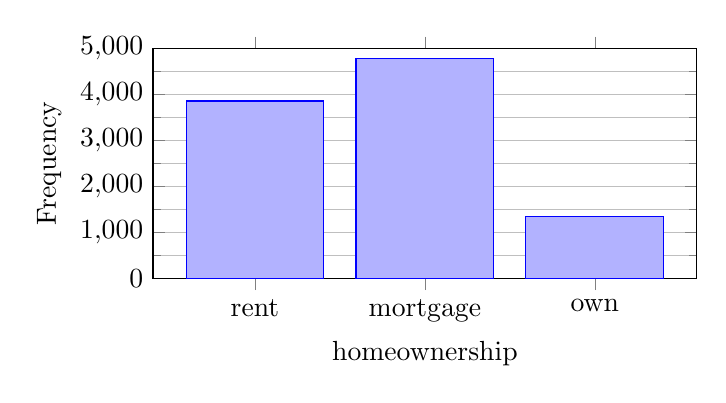
\begin{tikzpicture}
\begin{axis}[
height=4.5cm,
width=0.7\textwidth,
enlarge x limits=0.3,
ymajorgrids=true,
minor y tick num=1,
yminorgrids=true,
ylabel={Frequency},
xlabel={\variable{homeownership}},
bar width=1.75cm,
symbolic x coords={rent, mortgage, own},
ybar,
ymin=0,
ymax=5000,
ytick={0,1000,...,5000},
xtick=data,
xticklabel=\outcome{\tick},
]
\addplot+
coordinates
{
(rent, 3858)
(mortgage, 4789)
(own, 1353)
};
\end{axis}
\end{tikzpicture}
\end{center}
\end{example}\pause

\begin{note}
A histogram has no gaps between the bars, where as bar plot does.
\end{note}
\end{frame}

\begin{frame}
\begin{definition}
A bar plot that has been sorted so the largest bar is on the left and the smallest bar on the right is called \textbf{Pareto chart}.
\end{definition}\pause

\begin{example}
Here is the Pareto chart for the bar plot in Example~\ref{bar example 1}.
\begin{center}
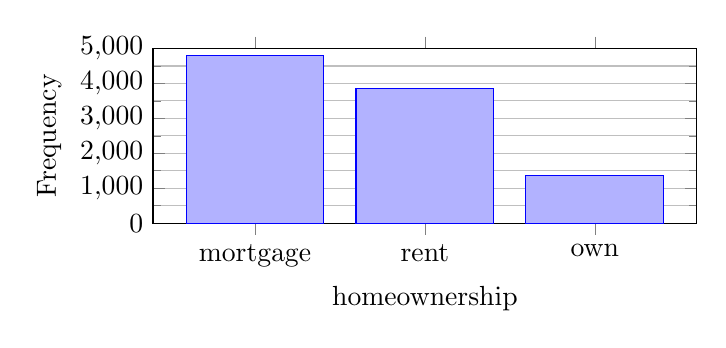
\begin{tikzpicture}
\begin{axis}[
height=3.8cm,
width=0.7\textwidth,
enlarge x limits=0.3,
ymajorgrids=true,
minor y tick num=1,
yminorgrids=true,
ylabel={Frequency},
xlabel={\variable{homeownership}},
bar width=1.75cm,
symbolic x coords={mortgage, rent, own},
ybar,
ymin=0,
ymax=5000,
ytick={0,1000,...,5000},
xtick=data,
xticklabel=\outcome{\tick},
]
\addplot+
coordinates
{
(mortgage, 4789)
(rent, 3858)
(own, 1353)
};
\end{axis}
\end{tikzpicture}
\end{center}
\end{example}\pause

\begin{note}
Named after Vilfredo Pareto, a noted Italian economist.
\end{note}
\end{frame}

\begin{frame}
\begin{note}
Instead of using frequencies, we could instead use proportions.
\end{note}\pause

\begin{example}
To find the proportion, divide each frequency by the total count.
\begin{center}
\renewcommand{\arraystretch}{2.2}
\begin{tabular}{lcc}\hline
\variable{homeownership} & Frequency & Proportion \\\hline
\outcome{rent} & 3858 & \visible<3->{$\dfrac{3858}{10000}=0.3858$} \\
\outcome{mortgage} & 4789 & \visible<4->{$\dfrac{4789}{10000}=0.4789$} \\
\outcome{own} & 1353 & \visible<5->{$\dfrac{1353}{10000}=0.1353$} \\[1mm]\hline
Total & 10000 & \visible<6->{$1.0000$} \\\hline
\end{tabular}
\end{center}
\end{example}
\end{frame}

\begin{frame}
\begin{example}
Here are both the frequency and proportion for \texttt{homeownership}.
\begin{center}
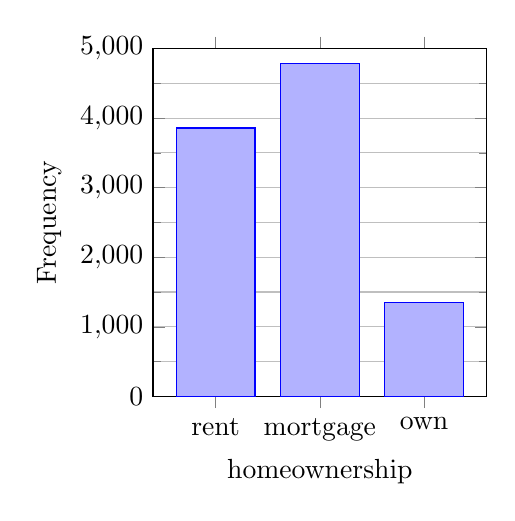
\begin{tikzpicture}
\begin{axis}[
height=6.0cm,
width=0.48\textwidth,
enlarge x limits=0.3,
ymajorgrids=true,
minor y tick num=1,
yminorgrids=true,
ylabel={Frequency},
xlabel={\variable{homeownership}},
bar width=1cm,
symbolic x coords={rent, mortgage, own},
ybar,
ymin=0,
ymax=5000,
ytick={0,1000,...,5000},
xtick=data,
xticklabel=\outcome{\tick},
]
\addplot+
coordinates
{
(rent, 3858)
(mortgage, 4789)
(own, 1353)
};
\end{axis}
\end{tikzpicture}
%
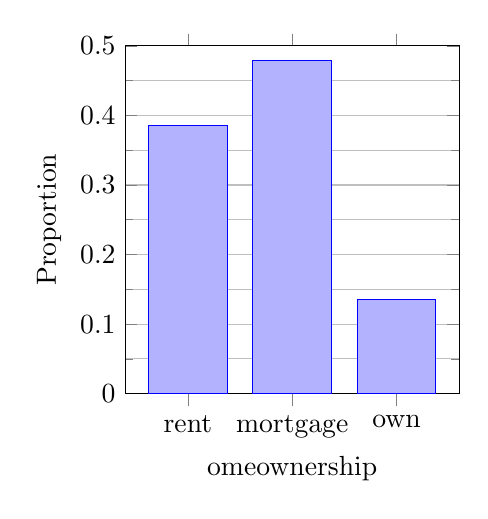
\begin{tikzpicture}
\begin{axis}[
height=6.0cm,
width=0.48\textwidth,
enlarge x limits=0.3,
ymajorgrids=true,
minor y tick num=1,
yminorgrids=true,
ylabel={Proportion},
xlabel={\variable{omeownership}},
bar width=1cm,
symbolic x coords={rent, mortgage, own},
ybar,
ymin=0,
ymax=0.5,
ytick={0,0.1,...,0.6},
xtick=data,
xticklabel=\outcome{\tick},
]
\addplot+
coordinates
{
(rent, 0.3858)
(mortgage, 0.4789)
(own, 0.1353)
};
\end{axis}
\end{tikzpicture}
\end{center}
\end{example}
\end{frame}

\begin{frame}
\begin{example}
Here, we use the \textbf{row proportions} for the contingency table from Example~\ref{contingency table}. Where we divide each count by their row total.
\begin{center}
\begin{tabular}{llcccc}
&&\multicolumn{3}{c}{\variable{homeownership}} &\\\cline{3-5}
&&\outcome{rent}&\outcome{mortgage}&\outcome{own}&Total\\\cline{2-6}
\multirow{2}{*}{{\variable{app\_type}}} & \outcome{individual} & 3496 & 3839 & 1170 & 8505 \\
&\outcome{joint} & 362 & 950 & 183 & 1495 \\\cline{2-6}
&Total & 3858 & 4789 & 1353 & 10000 \\\cline{2-6}
&&&$\downarrow~\downarrow~\downarrow$\\
&&\multicolumn{3}{c}{\variable{homeownership}} &\\\cline{3-5}
&&\outcome{rent}&\outcome{mortgage}&\outcome{own}&Total\\\cline{2-6}
\multirow{2}{*}{{\variable{app\_type}}} & \outcome{individual} & 0.4111 & 0.4514 & 0.1376 & 1.0000 \\
&\outcome{joint} & 0.2421 & 0.6355 & 0.1224 & 1.0000 \\\cline{2-6}
&Total & 0.3858 & 0.4789 & 0.1353 & 1.0000 \\\cline{2-6}
\end{tabular}
\end{center}\pause
\question{What does the number 0.4111 represent?}\pause
\answer{That $41.11\%$ of those that applied as individuals are renters.}
\end{example}
\end{frame}

\begin{frame}
\begin{example}\label{column proportion}
\vspace{-2mm}%beamer bug: extra space is added when a label is used, so this is to make this slide and the next look the same
Here, we use the \textbf{column proportions} for the contingency table from Example~\ref{contingency table}. Where we divide each count by their column total.
\begin{center}
\begin{tabular}{llcccc}
&&\multicolumn{3}{c}{\variable{homeownership}} &\\\cline{3-5}
&&\outcome{rent}&\outcome{mortgage}&\outcome{own}&Total\\\cline{2-6}
\multirow{2}{*}{{\variable{app\_type}}} & \outcome{individual} & 3496 & 3839 & 1170 & 8505 \\
&\outcome{joint} & 362 & 950 & 183 & 1495 \\\cline{2-6}
&Total & 3858 & 4789 & 1353 & 10000 \\\cline{2-6}
&&&$\downarrow~\downarrow~\downarrow$\\
&&\multicolumn{3}{c}{\variable{homeownership}} &\\\cline{3-5}
&&\outcome{rent}&\outcome{mortgage}&\outcome{own}&Total\\\cline{2-6}
\multirow{2}{*}{{\variable{app\_type}}} & \outcome{individual} & 0.9062 & 0.8016 & 0.8647 & 0.8505 \\
&\outcome{joint} & 0.0946 & 0.1984 & 0.1353 & 0.1495 \\\cline{2-6}
&Total & 1.0000 & 1.0000 & 1.0000 & 1.0000 \\\cline{2-6}
\end{tabular}
\end{center}\pause
\question{What does the number 0.9062 represent?}\pause
\answer{That $90.62\%$ of renters applied as individuals.}
\end{example}
\end{frame}

\begin{frame}
\begin{example}
Let us look at the column proportions from Example~\ref{column proportion} more closely.
\begin{center}
\vspace{-2mm}
\begin{tabular}{llcccc}
&&\multicolumn{3}{c}{\variable{homeownership}} &\\\cline{3-5}
&&\outcome{rent}&\outcome{mortgage}&\outcome{own}&Total\\\cline{2-6}
\multirow{2}{*}{{\variable{app\_type}}} & \outcome{individual} & 0.9062 & 0.8016 & 0.8647 & 0.8505 \\
&\outcome{joint} & 0.0946 & 0.1984 & 0.1353 & 0.1495 \\\cline{2-6}
&Total & 1.0000 & 1.0000 & 1.0000 & 1.0000 \\\cline{2-6}
\end{tabular}
\end{center}\pause
Notice that 90.62\% of renters applied as individuals, which is higher than for those with mortgages (80.16\%) or those who own (86.47\%).\pause

\vspace{1mm}
Because these rates vary between the three levels of \variable{homeowndership} (\outcome{rent}, \outcome{mortgage}, \outcome{own}), there is evidence that the \variable{app\_type} and \variable{homeownsership} variables are associated.
\end{example}\pause

\begin{note}
If we had considered row proportions instead, we would look down columns to see if the fraction of loans where the borrower rents, has a mortgage, or owns varied across the \outcome{individual} to \outcome{joint} types.
\end{note}
\end{frame}

\begin{frame}
\begin{example}\label{spam email}
\vspace{-2mm}%beamer bug: extra space is added when a label is used, so this is to make this slide and the next look the same
Data scientists use statistics to filter spam from incoming email messages. By noting specific characteristics of an email, an email may be classified as spam or not spam.\pause

\vspace{1mm}
One such characteristic is the email format, which indicates whether or not an email has any HTML content, such as bolded text. 
\only<2| handout:0>{%
\begin{center}\small
\begin{tabular}{lccc}\hline
&\outcome{text} & \outcome{HTML} & Total \\\hline
\outcome{spam} & 209 & 158 & 367 \\
\outcome{not spam} & 986 & 2568 & 2554 \\\hline
Total & 1195 & 2726 & 3921 \\\hline
\end{tabular}
\end{center}
}
%
\only<3->{%
\begin{center}\small
\begin{tabular}{lcccclccc}\cline{1-4}\cline{6-9}
&\outcome{text} & \outcome{HTML} & Total & & &\outcome{text} & \outcome{HTML} & Total \\\cline{1-4}\cline{6-9}
\outcome{spam} & 209 & 158 & 367 && \outcome{spam} & 0.175 & 0.058 & 0.094 \\
\outcome{not spam} & 986 & 2568 & 2554 && \outcome{not spam} & 0.825 & 0.942 & 0.651 \\\cline{1-4}\cline{6-9}
Total & 1195 & 2726 & 3921 && Total & 1.000 & 1.000 & 1.000 \\\cline{1-4}\cline{6-9}
\end{tabular}
\end{center}
}\pause

If we generate column proportions, we can see that a higher fraction of plain text emails are spam $\left(17.5\%\right)$ than compared to HTML emails $\left(5.8\%\right)$.\pause

\vspace{2mm}
But, this information is not enough on its own to classify an email and \outcome{spam} or \outcome{not spam}, since more than $80\%$ of plain text emails are not spam.
\end{example}
\end{frame}

\begin{frame}
\begin{definition}
A \textbf{stacked bar plot} is a graphical display of contingency tables.
\end{definition}

\begin{example}
\begin{center}
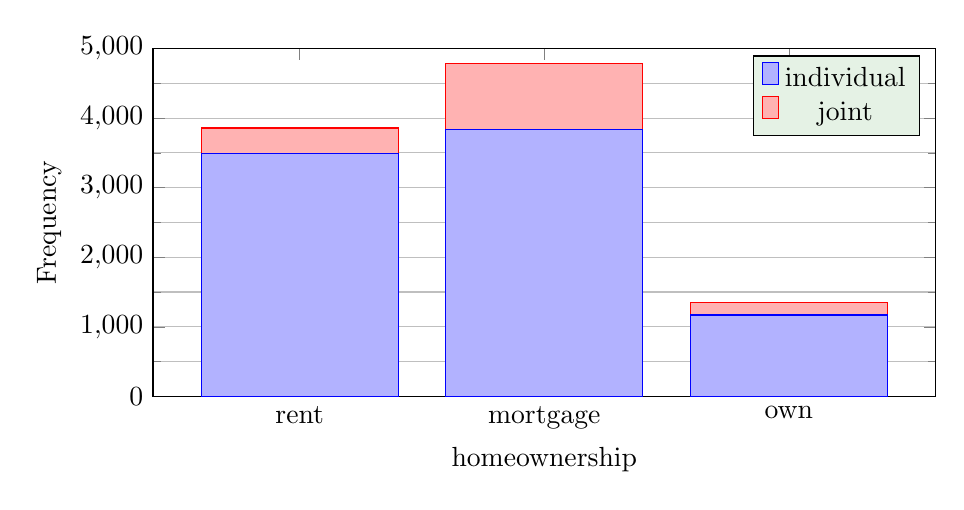
\begin{tikzpicture}
\begin{axis}[
height=6.0cm,
width=0.95\textwidth,
enlarge x limits=0.3,
ymajorgrids=true,
minor y tick num=1,
yminorgrids=true,
ylabel={Frequency},
xlabel={\variable{homeownership}},
bar width=2.5cm,
symbolic x coords={rent, mortgage, own},
ybar stacked,
ymin=0,
ymax=5000,
ytick={0,1000,...,5000},
xtick=data,
xticklabel=\outcome{\tick},
legend style={fill=legend, fill opacity=1},
]
\addplot+
coordinates
{
(rent, 3496)
(mortgage, 3839)
(own, 1170)
};
\addlegendentry{\outcome{individual}};
\addplot+
coordinates
{
(rent, 362)
(mortgage, 950)
(own, 183)
};
\addlegendentry{\outcome{joint}};
\end{axis}
\end{tikzpicture}
\end{center}
\end{example}
\end{frame}

\begin{frame}
\begin{definition}
A stacked bar plot generated from column proportions is called a \textbf{standardized stacked bar plot}.
\end{definition}

\begin{example}
\begin{center}
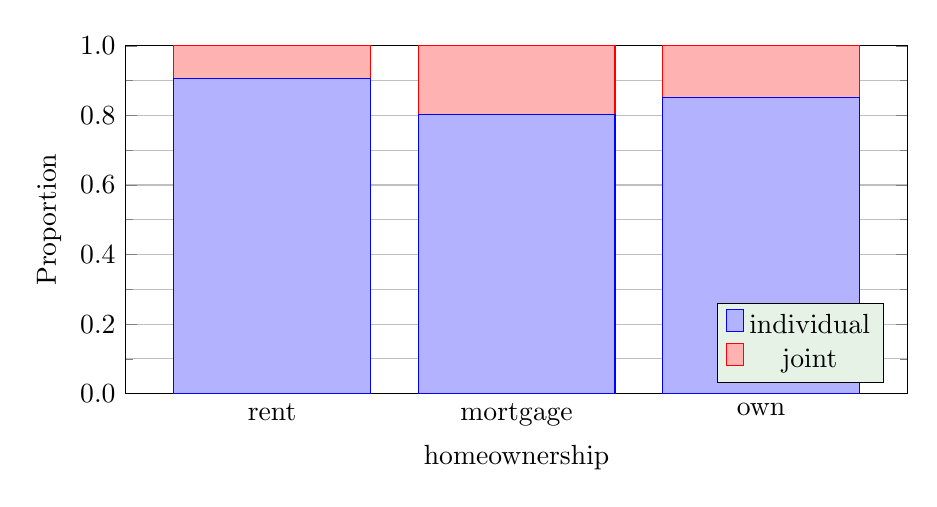
\begin{tikzpicture}
\begin{axis}[
height=6.0cm,
width=0.95\textwidth,
enlarge x limits=0.3,
ymajorgrids=true,
minor y tick num=1,
yminorgrids=true,
ylabel={Proportion},
xlabel={\variable{homeownership}},
bar width=2.5cm,
symbolic x coords={rent, mortgage, own},
ybar stacked,
ymin=0,
ymax=1,
ytick={0,0.2,...,1.1},
xtick=data,
xticklabel=\outcome{\tick},
legend pos = south east,
legend style={fill=legend, fill opacity=1},
y tick label style={
        /pgf/number format/.cd,
        fixed,
        fixed zerofill,
        precision=1,
        /tikz/.cd
    }
]
\addplot+
coordinates
{
(rent, 0.906)
(mortgage, 0.802)
(own, 0.851)
};
\addlegendentry{\outcome{individual}};
\addplot+
coordinates
{
(rent, 0.094)
(mortgage, 0.198)
(own, 0.150)
};
\addlegendentry{\outcome{joint}};
\end{axis}
\end{tikzpicture}
\end{center}
\end{example}
\end{frame}

\begin{frame}
\begin{definition}
A \textbf{side-by-side bar plot} is graphical display of contingency tables.
\end{definition}

\begin{example}
\begin{center}
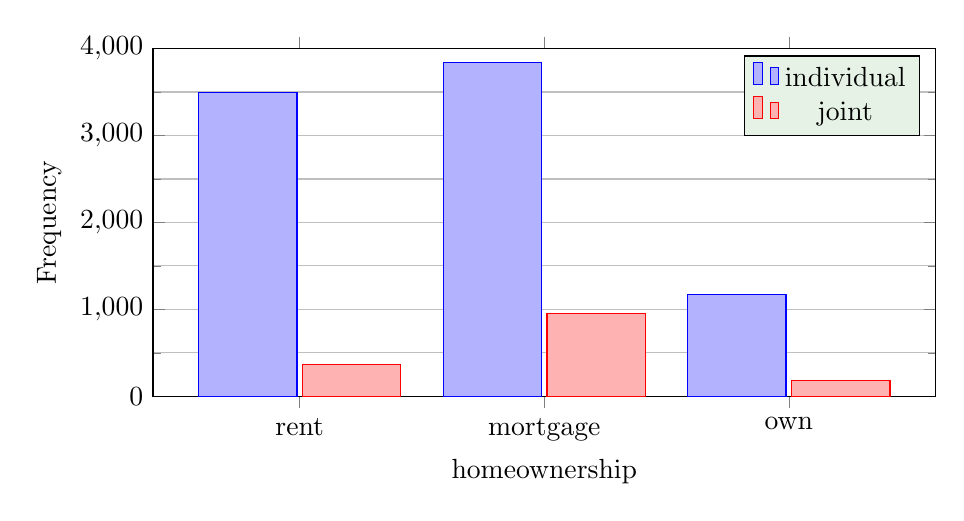
\begin{tikzpicture}
\begin{axis}[
height=6.0cm,
width=0.95\textwidth,
enlarge x limits=0.3,
ymajorgrids=true,
minor y tick num=1,
yminorgrids=true,
ylabel={Frequency},
xlabel={\variable{homeownership}},
bar width=1.25cm,
symbolic x coords={rent, mortgage, own},
ybar,
ymin=0,
ymax=4000,
ytick={0,1000,...,5000},
xtick=data,
xticklabel=\outcome{\tick},
legend style={fill=legend, fill opacity=1},
]
\addplot+
coordinates
{
(rent, 3496)
(mortgage, 3839)
(own, 1170)
};
\addlegendentry{\outcome{individual}};
\addplot+
coordinates
{
(rent, 362)
(mortgage, 950)
(own, 183)
};
\addlegendentry{\outcome{joint}};
\end{axis}
\end{tikzpicture}
\end{center}
\end{example}
\end{frame}

\begin{frame}
\begin{note}
The stacked bar plot is most useful when it's reasonable to assign one variable as the explanatory variable and the other variable as the response.
\end{note}\pause

\begin{note}
Side-by-side bar plots are more agnostic in their display about which variable, if any, represents the explanatory variable and which the response variable.
\end{note}\pause

\begin{note}
The standardized stacked bar plot is useful when the primary variable in the stacked bar plot is relatively imbalanced.
\end{note}
\end{frame}

\begin{frame}
\begin{note}
When a group of bars have very different sizes, relative to the other groups, it is difficult to discern if there is an association between the variables.
\end{note}\pause

\begin{example}
\begin{center}
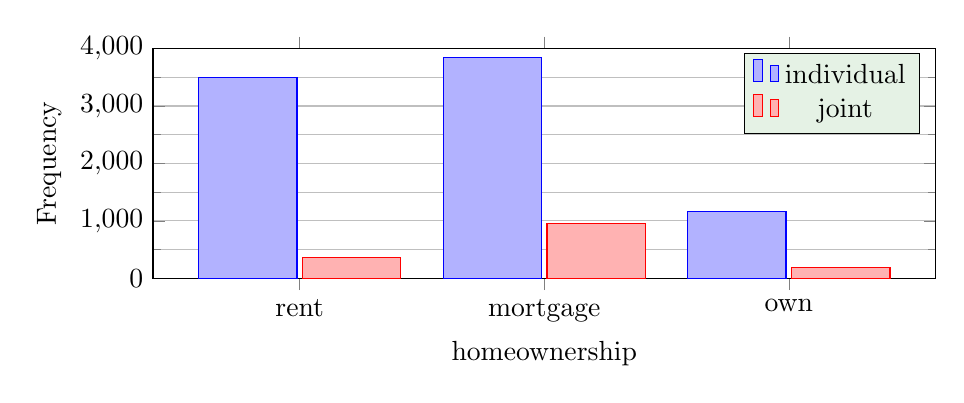
\begin{tikzpicture}
\begin{axis}[
height=4.5cm,
width=0.95\textwidth,
enlarge x limits=0.3,
ymajorgrids=true,
minor y tick num=1,
yminorgrids=true,
ylabel={Frequency},
xlabel={\variable{homeownership}},
bar width=1.25cm,
symbolic x coords={rent, mortgage, own},
ybar,
ymin=0,
ymax=4000,
ytick={0,1000,...,5000},
xtick=data,
xticklabel=\outcome{\tick},
legend style={fill=legend, fill opacity=1},
]
\addplot+
coordinates
{
(rent, 3496)
(mortgage, 3839)
(own, 1170)
};
\addlegendentry{\outcome{individual}};
\addplot+
coordinates
{
(rent, 362)
(mortgage, 950)
(own, 183)
};
\addlegendentry{\outcome{joint}};
\end{axis}
\end{tikzpicture}
\end{center}

\vspace{-4mm}
The bars for the \outcome{own} group are both much shorter than the other bars, so you can't tell from this plot if there is an association.
\end{example}
\end{frame}

\begin{frame}
\begin{note}
A standardized stacked bar plot is useful for checking for association.
\end{note}

\begin{example}
\begin{center}
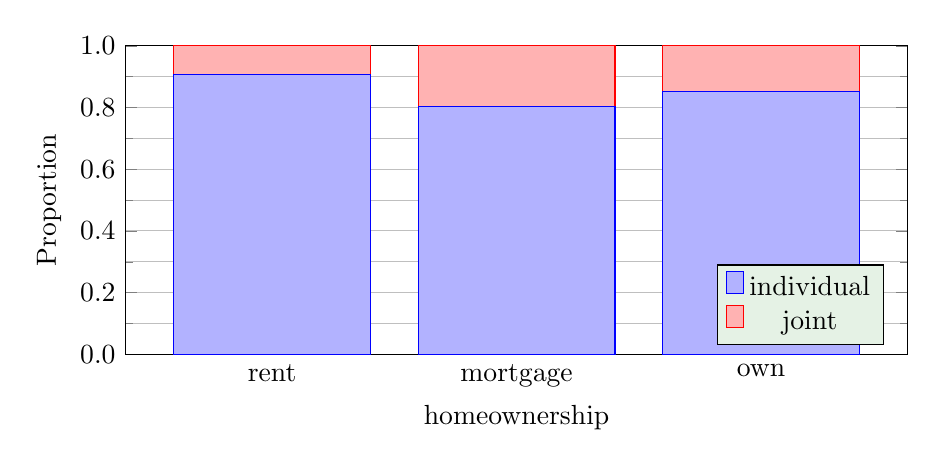
\begin{tikzpicture}
\begin{axis}[
height=5.5cm,
width=0.95\textwidth,
enlarge x limits=0.3,
ymajorgrids=true,
minor y tick num=1,
yminorgrids=true,
ylabel={Proportion},
xlabel={\variable{homeownership}},
bar width=2.5cm,
symbolic x coords={rent, mortgage, own},
ybar stacked,
ymin=0,
ymax=1,
ytick={0,0.2,...,1.1},
xtick=data,
xticklabel=\outcome{\tick},
legend pos = south east,
legend style={fill=legend, fill opacity=1},
y tick label style={
        /pgf/number format/.cd,
        fixed,
        fixed zerofill,
        precision=1,
        /tikz/.cd
    }
]
\addplot+
coordinates
{
(rent, 0.906)
(mortgage, 0.802)
(own, 0.851)
};
\addlegendentry{\outcome{individual}};
\addplot+
coordinates
{
(rent, 0.094)
(mortgage, 0.198)
(own, 0.150)
};
\addlegendentry{\outcome{joint}};
\end{axis}
\end{tikzpicture}
\end{center}

\vspace{-4mm}
Since the proportions vary for each outcome of \variable{homeownership}, there is an association.
\end{example}
\end{frame}

\begin{frame}
\begin{example}
Suppose grade school students were surveyed and asked which of the following they though was the most important: grades, popularity, sports. \pause

\vspace{1mm}
The standardized stacked bar plot represents the responses.
\begin{center}
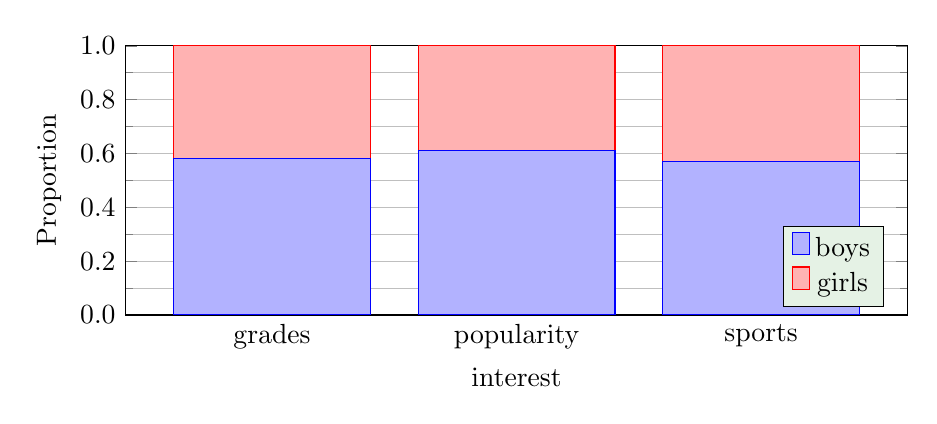
\begin{tikzpicture}
\begin{axis}[
height=5.0cm,
width=0.95\textwidth,
enlarge x limits=0.3,
ymajorgrids=true,
minor y tick num=1,
yminorgrids=true,
ylabel={Proportion},
xlabel={\variable{interest}},
bar width=2.5cm,
symbolic x coords={grades, popularity, sports},
ybar stacked,
ymin=0,
ymax=1,
ytick={0,0.2,...,1.1},
xtick=data,
xticklabel=\outcome{\tick},
legend pos = south east,
legend style={fill=legend, fill opacity=1},
y tick label style={
        /pgf/number format/.cd,
        fixed,
        fixed zerofill,
        precision=1,
        /tikz/.cd
    }
]
\addplot+
coordinates
{
(grades, 0.58)
(popularity, 0.61)
(sports, 0.57)
};
\addlegendentry{\outcome{boys}};
\addplot+
coordinates
{
(grades, 0.42)
(popularity, 0.39)
(sports, 0.43)
};
\addlegendentry{\outcome{girls}};
\end{axis}
\end{tikzpicture}
\end{center}

\vspace{-4mm}
Since the proportions do not significantly vary for each outcome, the variables \variable{gender} and \variable{interest} are independent.
\end{example}
\end{frame}

\begin{frame}
\begin{note}
To compare numerical and categorical variable, you can group the numbers based on the possible outcomes of the categorical variable, then draw a plot for each group.
\end{note}\pause

\begin{example}
If we wish to compare the median income to whether a county gained population, we could build the table.

\vspace{-1mm}
\begin{center}
\begin{tabular}{cccccccccc}
\multicolumn{10}{c}{Median Income for U.S. Counties, in \$1000s}\\\hline
\multicolumn{6}{c}{Population Gain} && \multicolumn{3}{c}{No Population Gain}\\\cline{1-6}\cline{8-10}
38.2&43.6&42.2&61.5&51.1&45.7&&48.3&60.3&50.7\\
38.2&43.6&44.6&51.8&40.6&63.3&&48.3&60.3&50.7\\
51.1&34.1&80.8&46.3&75.2&40.6&&39.3&40.4&40.3\\
51.9&34.7&61.0&51.4&53.8&57.6&&57.0&47.2&45.9\\
53.1&54.6&63.0&49.1&46.6&46.5&&42.3&41.5&46.1\\
74.2&63.0&63.2&47.6&50.4&49.0&&44.9&51.7&46.4\\
$\vdots$&$\vdots$&$\vdots$&$\vdots$&$\vdots$&$\vdots$&&$\vdots$&$\vdots$&$\vdots$
\end{tabular}
\end{center}
\end{example}
\end{frame}

\begin{frame}
\begin{definition}
A \textbf{frequency polygon} or \textbf{hollow histogram} allows us to compare numerical and categorical variables. It uses line segments connected to points located where the top of the bar would be. 
\end{definition}\pause
\begin{example}
The plot shows the wait times for both McDonald's and Dunkin' Donuts.
\begin{center}
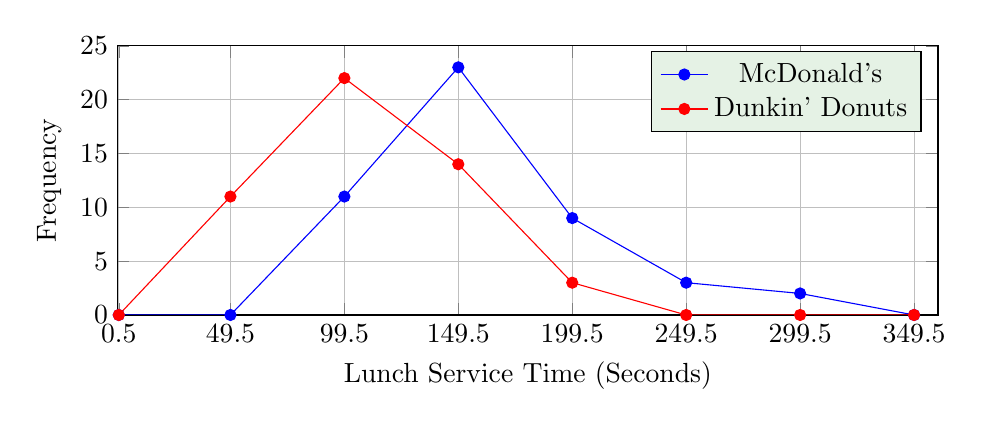
\begin{tikzpicture}
\begin{axis}[
width=12cm,
height=5.0cm,
xlabel={Lunch Service Time (Seconds)},
ylabel={Frequency},
ytick={0,5,...,25},
xtick=data,%{24.5,49.5,99.5,...,349.5},
ymajorgrids=true,
xmajorgrids=true,
ymin=0,
ymax=25,
xmin=0,
xmax=360,
scatter/use mapped color={
 %draw=mapped color,
 %fill=blue,
},
legend style={fill=legend, fill opacity=1}
]
\addplot[scatter, blue, scatter src=y]
coordinates
{
(0.5, 0)
(49.5, 0)
(99.5, 11) 
(149.5, 23)
(199.5, 9)
(249.5, 3)
(299.5, 2)
(349.5, 0)
};
\addlegendentry{McDonald's}

\addplot[scatter, red, scatter src=y]
coordinates
{
(0.5, 0)
(49.5, 11)
(99.5, 22) 
(149.5, 14)
(199.5, 3)
(249.5, 0)
(299.5, 0)
(349.5, 0)
};
\addlegendentry{Dunkin' Donuts}
\end{axis}
\end{tikzpicture}
\end{center}
\end{example}
\end{frame}

\begin{frame}
\begin{note}
For small data sets (20 values or fewer), use a table instead of a graph.
\end{note}\pause

\begin{note}
A graph of data should draw focus to the true nature of the data, not on other elements, such as eye-catching but distracting design features.
\end{note}\pause

\begin{note}
Do not distort data. Construct a graph to reveal the true nature of the data.
\end{note}\pause

\begin{note}
Almost all of the ink in a graph should be used for data, not for other design elements.
\end{note}
\end{frame}

\begin{frame}
\begin{note}
Always examine a graph carefully to see whether a vertical axis begins at some point other than zero so that differences are exaggerated.
\end{note}\pause

\begin{example}
\begin{center}
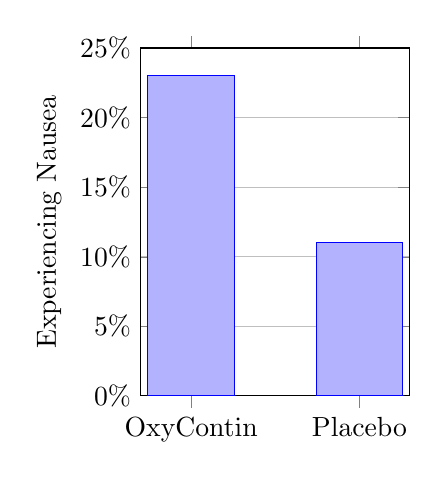
\begin{tikzpicture}
\begin{axis}[
height=6.0cm,
width=5.0cm,
enlarge x limits=0.3,
ymajorgrids=true,
ylabel={Experiencing Nausea},
xlabel={},
bar width=1.1cm,
symbolic x coords={OxyContin, Placebo},
ybar,
ymin=0,
ymax=25,
ytick={0,5,...,25},
xtick=data,
yticklabel style={/pgf/number format/.cd,fixed,precision=0},
yticklabel=
\pgfmathprintnumber\tick\%
]
\addplot+
coordinates
{
(OxyContin, 23)
(Placebo, 11)
};
\end{axis}
\end{tikzpicture}
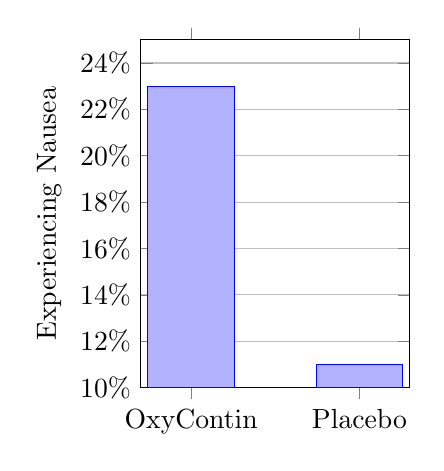
\begin{tikzpicture}
\begin{axis}[
height=6.0cm,
width=5.0cm,
enlarge x limits=0.3,
ymajorgrids=true,
ylabel={Experiencing Nausea},
xlabel={},
bar width=1.1cm,
symbolic x coords={OxyContin, Placebo},
ybar,
ymin=10,
ymax=25,
ytick={10,12,...,24},
xtick=data,
yticklabel style={/pgf/number format/.cd,fixed,precision=0},
yticklabel=
\pgfmathprintnumber\tick\%
]
\addplot+
coordinates
{
(OxyContin, 23)
(Placebo, 11)
};
\end{axis}
\end{tikzpicture}
\end{center}
\end{example}
\end{frame}

\begin{frame}
\begin{note}
When examining data depicted with a pictograph, beware when area or volume is used to depict amounts that are actually one-dimensional.
\end{note}\pause

\begin{example}
The pictographs show data from the CDC\@.

\vspace{-7mm}
\begin{figure}
\centering
\hfill
\subfigure[1970: 36\% of U.S. adults smoked.]{\includegraphics[width=.44\textwidth]{Cigarette.png}}
\hfill
\subfigure[2013: 18\% of U.S. adults smoked.]{\includegraphics[width=.44\textwidth]{Cigarette_small.png}}
\hfill
\end{figure}
The larger cigarette is about twice as long as the smaller, which means it has four times the area of the smaller cigarette. While the data shows that 36\% is only double 18\%.
\end{example}
\end{frame}

\begin{frame}
\begin{definition}
A \textbf{pie chart} is a worse version of the bar chart.
\begin{center}
\includegraphics[width=0.8\textwidth]{zoidberg.jpg}
\end{center}
\end{definition}
\end{frame}

\begin{frame}
\begin{example}
\begin{center}
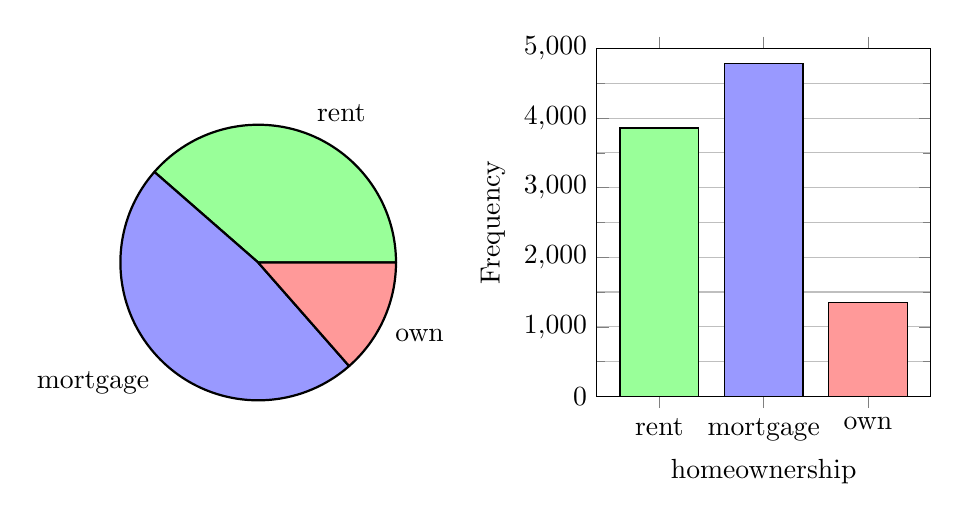
\begin{tikzpicture}
\pie[
radius=1.75,
hide number,
pos={-4.3,1.7},
color={green!40, blue!40, red!40},
]
{38.58/\outcome{rent},
47.89/\outcome{mortgage},
13.53/\outcome{own}}
\begin{axis}[
height=6.0cm,
width=0.48\textwidth,
enlarge x limits=0.3,
ymajorgrids=true,
minor y tick num=1,
yminorgrids=true,
ylabel={Frequency},
xlabel={\variable{homeownership}},
bar width=1cm,
symbolic x coords={rent, mortgage, own},
ybar,
ymin=0,
ymax=5000,
ytick={0,1000,...,5000},
xtick={rent, mortgage, own},
xticklabel=\outcome{\tick},
every axis plot/.append style={
          bar shift=0pt,
        }
]
\addplot+[draw=black, fill=green!40] coordinates{(rent, 3858)};
\addplot+[draw=black, fill=blue!40] coordinates{(mortgage, 4789)};
\addplot+[draw=black, fill=red!40] coordinates{(own, 1353)};
\end{axis}
\end{tikzpicture}
\end{center}
The pie chart makes it harder to tell the relative sizes of each group, where the bar plot makes it much easier and gives the actual frequencies.
\end{example}
\end{frame}
\end{document}
